\section{L'algoritmo di Hough per curve ad S}
\subsection{Parametrizzazione della curva}
Come anticipato nell'introduzione, la prima cosa da fare è determinare quale forma analitica vogliamo andare ad individuare nell'immagine.\par
Prendiamo una sigmoide semplice centrata in $(0,\ 0)$:
$$y(x)=\frac{e^x}{1+e^x}-0.5$$
\begin{center}
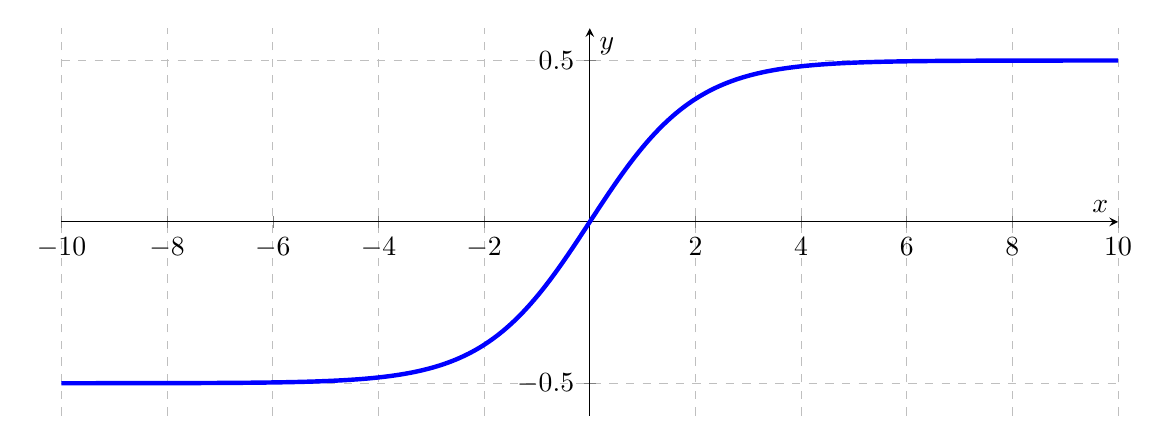
\begin{tikzpicture}
\begin{axis}[
    axis lines = middle,
    xlabel = \( x \),
    ylabel = \( y \),
    xmin = -10, xmax = 10,
    ymin = -0.6, ymax = 0.6,
    width = 15cm, height = 6.5cm,
    grid = both,
    grid style = {dashed, gray!50},
    samples = 1000,
    domain = -10:10
]
\addplot[blue, ultra thick] {exp(x)/(1+exp(x))-0.5};
\end{axis}
\end{tikzpicture}
\end{center}

Questa curva si adatta perfettamente alle necessità che abbiamo. Adesso dobbiamo gestirne la velocità con cui passa dall'asintoto inferiore a quello superiore e l'ampiezza, in modo da poter generare tutte le curve di interesse.\par
Il primo parametro lo chiamiamo $a$ ed il secondo $d$, adesso la formula diventa:

$$y(x)=d\cdot\bigg(\frac{e^{a\cdot x}}{1+e^{a\cdot x}}-0.5\bigg)$$
\begin{center}
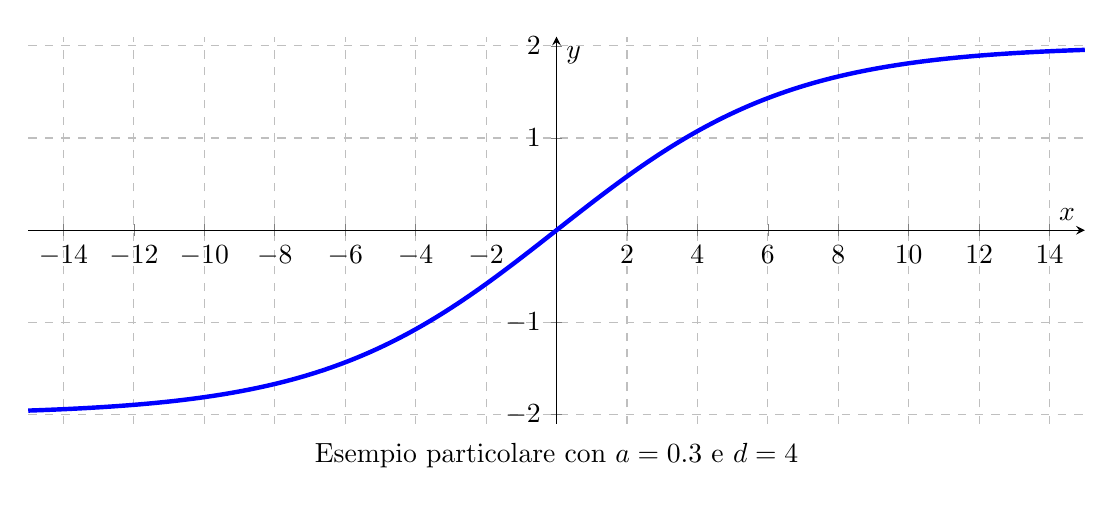
\begin{tikzpicture}
\begin{axis}[
    axis lines = middle,
    xlabel = \( x \),
    ylabel = \( y \),
    xmin = -15, xmax = 15,
    ymin = -2.1, ymax = 2.1,
    width = 15cm, height = 6.5cm,
    grid = both,
    grid style = {dashed, gray!50},
    samples = 1000,
    domain = -15:15
]
\addplot[blue, ultra thick] {4*(exp(0.3*x)/(1+exp(0.3*x))-0.5)};
\end{axis}
\node[align=center, below] at (current bounding box.south) {Esempio particolare con $a = 0.3$ e $d = 4$};
\end{tikzpicture}
\end{center}

\newpage

\subsection{Trasposizione dell'algoritmo}
L'\hyperref[lst:ostinelli_Tensore4]{algoritmo} a pagina seguente,  genera tutte le curve con parametri $a$ e $d$ in range prestabiliti. Data la complessità computazionale dell'algoritmo può avere senso, dove è concesso, limitare i domini di $a$ e $d$ per generare e quindi testare meno curve. Ad esempio, volessimo solo curve con derivata prima positiva, basterebbe mantenere $a>0$.\par
Una volta generata una curva, che chiameremo $S$, sovrapponiamo, per ogni pixel di riga $c$, e di colonna $b$, la curva sull'immagine in modo che il suo centro coincida con il pixel.\par
A questo punto contiamo le occorrenze dei pixel neri in corrispondenza della curva, questo numero fornisce una misura della presenza della curva di centro $(c,\ b)$.

\subsection{Punti critici di questo approccio}
Il porting dell'algoritmo di Hough ci mette nelle condizioni di avere un tensore di accumulazione in quattro dimensioni. Questo è un problema poiché è molto complicato trovare un modo di rappresentare le cinque dimensioni in un modo comprensibile all'utente.\par
Disegnare un grafico in cinque dimensioni, rappresenta una sfida significativa a causa della complessità aggiuntiva nell'interpretazione visiva di più variabili. Mentre la rappresentazione di dati in due o tre dimensioni è relativamente intuitiva, aggiungere dimensioni comporta un aumento esponenziale della complessità percettiva.\par
La principale difficoltà risiede, quindi, nel trovare un metodo efficace per visualizzare in modo chiaro e comprensibile tutte e cinque le dimensioni simultaneamente. Le tradizionali tecniche di visualizzazione, come grafici a dispersione o grafici a barre, diventano rapidamente inefficienti e ingombranti con un numero così elevato di dimensioni. Altresì, la sovrapposizione di più informazioni sullo stesso grafico può portare a confusione e difficoltà nel distinguere tra i diversi elementi.\par
Un altro aspetto da tenere in considerazione è che, la memorizzazione di grandi quantità di dati in tensori, diventa computazionalmente più complesso man mano che le dimensioni dei dati aumentano. Questo perché l'aumento delle dimensioni comporta una crescita esponenziale del numero totale di elementi nel tensore.\par
Di conseguenza, viene limitata la capacità di elaborare immagini molto risolute, che a parità di dimensioni hanno molti più valori da salvare ed elaborare.

\newpage
\lstinputlisting[
    style=matlabStyle,
    caption={Pseudocodice per la trasformata di Hough per curve ad S},
    label={lst:ostinelli_Tensore4}
]{codici/Ostinelli_Tensore4.m}
\newpage